\section[Spontaneous Symmetry Breaking and Goldstone Theorem]{Spontaneous Symmetry Breaking and\\Goldstone Theorem}

It is straightforward to verify that the original unperturbed Hamiltonian commutes with the total number operator \( \hat{N} = \sum_{\mathbf{k}} a_{\mathbf{k}}^\dagger a_{\mathbf{k}} \). This commutation property is intimately connected with the fundamental invariance of the Hamiltonian under global \( \text{U}(1) \) phase transformations:
\[
    a_{\mathbf{k}} \to e^{i\phi} a_{\mathbf{k}},
\]
\[
    a_{\mathbf{k}}^\dagger \to e^{-i\phi} a_{\mathbf{k}}^\dagger.
\]
These phase rotations are formally realized by the application of the unitary continuous symmetry operator \( U(\phi) \):
\[
    U(\phi) = e^{i\phi\hat{N}}.
\]
Indeed, it is easy to explicitly check the generator action on the annihilation operator:
\[
    U^\dagger(\phi) a_{\mathbf{k}} U(\phi) = e^{i\phi} a_{\mathbf{k}}.
\]
Because the Hamiltonian is invariant under this specific transformation—meaning \( U^\dagger(\phi) H U(\phi) = H \)—Noether's theorem guarantees there should be a conserved macroscopic charge. This conserved charge is nothing else than the mathematical generator of the transformation itself, namely, the total number operator \( \hat{N} \).

Crucially, even if the Hamiltonian governing the system is perfectly invariant under the above \( \text{U}(1) \) transformation, the interacting ground state \( |\psi_0\rangle \) is not. This profound physical phenomenon is known as spontaneous symmetry breaking. There are multiple analytical ways to see this symmetry breaking. Consider the macroscopic expectation value of the zero-momentum annihilation operator \( a_0 \). We previously established that over the coherent ground state, \( \langle \psi_0 | a_0 | \psi_0 \rangle \neq 0 \). Applying the unitary transformation, we have:
\[
    \langle \psi_0 | (U^\dagger(\phi) a_0 U(\phi)) | \psi_0 \rangle = \langle \psi_0 | (e^{i\phi} a_0) | \psi_0 \rangle.
\]
However, if the ground state \( |\psi_0\rangle \) were truly invariant under the symmetry group, then by definition \( U(\phi) |\psi_0\rangle = |\psi_0\rangle \). This invariant assumption would require that the equation evaluates to:
\[
    \langle \psi_0 | a_0 | \psi_0 \rangle = e^{i\phi} \langle \psi_0 | a_0 | \psi_0 \rangle,
\]
which can logically be satisfied for an arbitrary phase \( \phi \) if and only if \( \langle \psi_0 | a_0 | \psi_0 \rangle = 0 \). This immediately leads to a direct contradiction with our foundational result that the condensate is macroscopically occupied. The exact same mathematical proof can be repeated for the pair correlation expectation value at finite momenta \( \mathbf{k} \neq 0 \). In that case, we notice that
\[
    \langle \psi_0 | a_{\mathbf{k}} a_{-\mathbf{k}} | \psi_0 \rangle = -u_k v_k \neq 0,
\]
and applying the operator \( U(\phi) \) to both bare operators and falsely imposing the invariance of the ground state \( |\psi_0\rangle \) once again yields a fatal contradiction.

\begin{figure}[H]
    \begin{minipage}{0.6\textwidth}
        \centering
        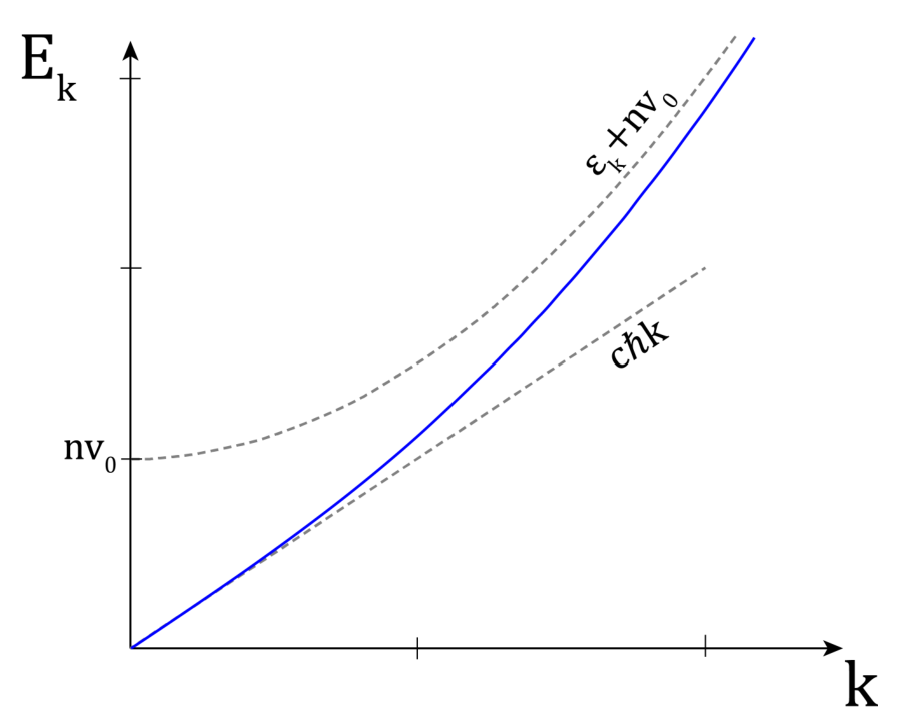
\includegraphics[width=0.8\linewidth]{img/1-dispersion_asymptotic.png}
    \end{minipage}
    \hfill
    \begin{minipage}{0.35\textwidth}
        \caption{Plot of the dispersion \( E_k = \sqrt{\epsilon_k^2 + 2nU_0\epsilon_k} \) (blue line) with its two asymptotic behaviours: for \( k \to 0 \) we have that the dispersion is linear with \( E_k \sim c\hbar k \), while for \( k \to \infty \) we have that the dispersion is quadratic with \( E_k \sim \epsilon_k + nU_0 \).}
        \label{fig:dispersion_asymptotic}
    \end{minipage}
\end{figure}

Once we have rigorously verified that the chosen ground state explicitly breaks the continuous \( \text{U}(1) \) symmetry, we know by Goldstone's theorem that there must emerge massless Goldstone bosons. These excitations must exhibit an energy dispersion that vanishes continuously (specifically, linearly) with the momentum \( p \), yielding \( E \sim cp \) for \( p \to 0 \). Recall that after executing the Bogoliubov transformation, the interacting Hamiltonian becomes diagonalized, featuring the quasiparticle energy spectrum given by \( E_k \). The asymptotic limit \( k \to 0 \) for \( E_k \) has been already evaluated, successfully reproducing exactly the linear phononic dispersion that Goldstone's theorem demands: \( E_k \sim c\hbar k \) (as visualized in Figure \ref{fig:dispersion_asymptotic}), with the characteristic sound velocity \( c \) scaling with the interaction strength.

\begin{figure}[H]
    \begin{minipage}{0.5\textwidth}
        \caption{Elementary excitations are modes that allow us to describe low energy states. If we excite the ground state GS, increasing the energy by \( +E_k \), it's like creating an elementary excitation (a quasi-particle).}
        \label{fig:elementary_excitations}
    \end{minipage}
    \hfill
    \begin{minipage}{0.45\textwidth}
        \centering
        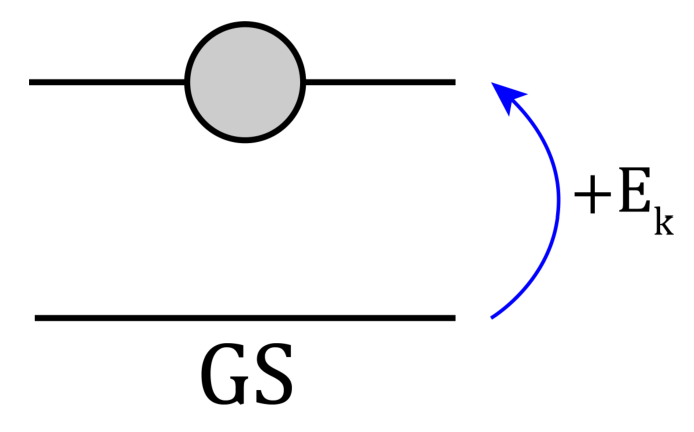
\includegraphics[width=0.9\linewidth]{img/1-elementary_excitations.png}
    \end{minipage}
\end{figure}

The derived energy values \( E_k \) structurally describe the dispersion of these elementary excitations, which are collective modes that allow us to describe effectively low-energy many-body states as a simple ideal gas of quasi-particles (see Figure \ref{fig:elementary_excitations}). This quasiparticle framework is particularly relevant at very low temperatures \( T \), when only these low-energy excited states are thermally activated, since random thermal fluctuations are small and strictly of order \( k_B T \).

Consequently, complex interacting states at low energy can be cleanly described as a dilute gas of elementary excitations. It is critical to recognize that these independent excitations are not the original bare bosons created by the standard operators \( a_{\mathbf{k}}^\dagger \), but rather new hybridized bosonic modes created by the Bogoliubov operators \( \alpha_{\mathbf{k}}^\dagger \) for small \( k \). These elementary excitations are governed by an effective interacting dispersion \( E_k \) that is structurally distinct from the purely quadratic free-particle dispersion \( \epsilon_k \) of the original bare bosons.

Remarkably, even for a strongly interacting bare Bose gas, provided the temperature remains sufficiently low, very few of these hybridized modes are activated. Because the thermal density of quasi-particles is low, these elementary excitations are highly dilute and can thus be treated to an excellent approximation as a non-interacting ideal gas. Lastly, we note a fundamental statistical constraint: for a system comprised exclusively of underlying bosons, like in the present model, only bosonic elementary excitations are physically possible. In contrast, for a many-body system of underlying fermions, the collective excitations can manifest as either fermionic (quasiparticles) or bosonic (e.g., Cooper pairs, plasmons) elementary excitations depending on the specific pairing mechanics.

\section{Specific Heat and Condensate Fraction}

Let us proceed with the calculation of the specific heat of a dilute Bose gas. From the diagonalized Hamiltonian, we established that at absolute zero temperature, \( T = 0 \), the system resides in the quasiparticle vacuum with no elementary excitations. At a finite temperature \( T > 0 \), the thermal mean number of elementary excitations, \( \langle \alpha_{\mathbf{k}}^\dagger \alpha_{\mathbf{k}} \rangle \), is governed by the standard Bose-Einstein distribution—since these Bogoliubov quasiparticles are fundamentally bosons:
\[
    \langle \alpha_{\mathbf{k}}^\dagger \alpha_{\mathbf{k}} \rangle = \frac{1}{e^{\beta E_k} - 1},
\]
where \( \beta = (k_B T)^{-1} \). In this expression, the chemical potential \( \mu \) associated with the elementary excitations is strictly zero. This physically arises because the total number of quasiparticle excitations is not a conserved quantity; it is determined dynamically by the thermal equilibrium at temperature \( T \) (entirely analogous to phonons in a crystalline solid or photons in black-body radiation). Consequently, the total internal energy \( E(T) \) of the gas at temperature \( T \) is given by the sum of the zero-point ground state energy and the thermal excitation energy:
\[
    E(T) = \mathcal{E}_0 + \sum_{\mathbf{k}} \frac{E_k}{e^{\beta E_k} - 1}.
\]
Taking the thermodynamic limit, the discrete summation over wave vectors transitions into a continuous integral, yielding the total energy density:
\[
    \frac{E(T)}{V} = \frac{\mathcal{E}_0}{V} + \int \frac{d^3k}{(2\pi)^3} \frac{E_k}{e^{\beta E_k} - 1}.
\]
For high-energy modes where \( E_k \gtrsim k_B T \), the integrand is exponentially suppressed by the Bose distribution. Therefore, the dominant contribution to the integral comes strictly from the low-energy domain where \( E_k \lesssim k_B T \). At very low temperatures, this restricts our focus to the extreme long-wavelength limit of the dispersion relation.

\begin{figure}[H]
    \begin{minipage}{0.6\textwidth}
        \centering
        \TODO{add image of a graph showing the quasiparticle dispersion energy curve plotted against momentum, with a highlighted circle near the origin emphasizing the linear regime at low energies comparable to thermal fluctuations}
    \end{minipage}
    \hfill
    \begin{minipage}{0.35\textwidth}
        \caption{At low temperature \( T \), if we are interested just in the region \( E_k \lesssim k_B T \), we can see that the dispersion \( E_k \) goes linearly with the momentum \( k \).}
        \label{fig:dispersion_lowT}
    \end{minipage}
\end{figure}

In this low-momentum regime, we recall that the Bogoliubov dispersion is strictly linear, \( E_k \approx c\hbar k \). Thus, in the asymptotic limit \( T \to 0 \), we can safely replace the full dispersion relation with its phononic approximation inside the integral:
\[
    \frac{E(T)}{V} = \frac{\mathcal{E}_0}{V} + \int \frac{d^3k}{(2\pi)^3} \frac{c\hbar k}{e^{\beta c\hbar k} - 1}.
\]
Evaluating this integral by switching to spherical coordinates and introducing the dimensionless integration variable \( x = \beta c\hbar k \), we obtain:
\[
    \begin{aligned}
        \frac{E(T)}{V} & = \frac{\mathcal{E}_0}{V} + \left(\frac{k_B T}{c\hbar}\right)^3 k_B T \frac{4\pi}{(2\pi)^3} \int_0^\infty \frac{x^3}{e^x - 1} dx \\
                       & = \frac{\mathcal{E}_0}{V} + \frac{\pi^2}{30} \frac{(k_B T)^4}{(c \hbar)^3}.
    \end{aligned}
\]

From this energy density, we directly compute the isochoric heat capacity, \( C_V \):
\[
    C_V = \left( \frac{\partial E(T)}{\partial T} \right)_V = \frac{2\pi^2}{15} V k_B \left( \frac{k_B T}{c\hbar} \right)^3.
\]

\begin{figure}[H]
    \begin{minipage}{0.35\textwidth}
        \caption{Plot of the behavior of the specific heat \( C_V \) at low temperature for a bosonic system. The blue line represents the specific heat of an interacting Bose gas, which scales proportionally to the cube of the temperature. The red line represents the specific heat of a non-interacting Bose gas, scaling proportionally to the temperature to the power of three halves.}
        \label{fig:specific_heat}
    \end{minipage}
    \hfill
    \begin{minipage}{0.6\textwidth}
        \centering
        \TODO{add image of a graph comparing two curves of specific heat against temperature, showing a cubic blue curve for the interacting gas and a three halves power red curve for the ideal gas}
    \end{minipage}
\end{figure}

This final expression reveals that the low-temperature specific heat of the weakly interacting Bose gas scales as \( T^3 \). This characteristic cubic temperature dependence mirrors the behavior of acoustic phonons in a Debye solid or photons in a cavity, fundamentally stemming from the linear phononic dispersion relation. We can starkly contrast this interacting result with the ideal, non-interacting Bose gas, which exhibits a \( T^{3/2} \) dependence due to its purely quadratic free-particle dispersion. In the interacting system, the linear dispersion creates a lower density of states at low energies compared to the non-interacting case, making the elementary excitations significantly harder to thermally excite at temperatures near absolute zero.

\section{Landau Criterion for Superfluidity}

 [...]